%
% IEEE Transactions on Microwave Theory and Techniques example
% Tibault Reveyrand - http://www.microwave.fr
%
% http://www.microwave.fr/LaTeX.html
% ---------------------------------------



% ================================================
% Please HIGHLIGHT the new inputs such like this :
% Text :
%  \hl{comment}
% Aligned Eq. 
% \begin{shaded}
% \end{shaded}
% ================================================

\documentclass[journal]{IEEEtran}

\renewcommand\thesection{\arabic{section}} 
\renewcommand\thesubsectiondis{\thesection.\arabic{subsection}}
\renewcommand\thesubsubsectiondis{\thesubsectiondis.\alph{subsubsection}}
\renewcommand\theparagraphdis{\arabic{paragraph}.}

%\usepackage[retainorgcmds]{IEEEtrantools}
%\usepackage{bibentry}  
\usepackage{xcolor,soul,framed} %,caption

\colorlet{shadecolor}{yellow}
% \usepackage{color,soul}
\usepackage[pdftex]{graphicx}
\graphicspath{{../pdf/}{../jpeg/}}
\DeclareGraphicsExtensions{.pdf,.jpeg,.png}

\usepackage[cmex10]{amsmath}
%Mathabx do not work on ScribTex => Removed
%\usepackage{mathabx}
\usepackage{array}
\usepackage{mdwmath}
\usepackage{mdwtab}
\usepackage{eqparbox}
\usepackage{url}

\hyphenation{op-tical net-works semi-conduc-tor}



%\bstctlcite{IEEE:BSTcontrol}
%=== TITLE & AUTHORS ====================================================================
\begin{document}
\bstctlcite{IEEEexample:BSTcontrol}
    \title{How can the effectiveness of marketing ‘Airbnb Seattle’ be improved?
– dataset of 2016 
}
  \author{LIST Nicole ,
      L\"OHR Tim,\\
      BOHNSTEDT Timo,
      PANG Tsz Ching,
      and~BAL Kiran Jeniffer% <-this % stops a space
}

% The paper headers
\markboth{Project Report
Machine Learning for Business IS4861 
}{Roberg \MakeLowercase{\textit{et al.}}: High-Efficiency Diode and Transistor Rectifiers}


% ====================================================================
\maketitle



% === ABSTRACT 
\begin{abstract}
%\boldmath
This paper presents a theoretical analysis of harmonically-terminated high-efficiency power rectifiers and experimental validation on a class-C single Schottky-diode rectifier and a class-F$^{\rm -1}$ GaN transistor rectifier. The theory is based on a Fourier analysis of current and voltage waveforms which arise across the rectifying element when different harmonic terminations are presented at its terminals. An analogy to harmonically-terminated power amplifier theory is discussed. From the analysis, one can obtain an optimal value for the DC load given the RF circuit design. An upper limit on rectifier efficiency is derivedce-pull measurement of a Schottky diode rectifier with short-circuit terminations at the second and third harmonic are presented. A maximal device rectification efficiency of 72.8 impedance for self-synchronous rectification. Measurements of conversion efficiency and output DC voltage for varying gate RF impedance, DC load and gate bias are shown with varying input RF power at the drain. The rectifier demonstrates an efficiency of 85\% for a 10\,W input RF power at the transistor drain, with a DC voltage of \hl{30\,V} across a 98\,$\Omega$ resistor.
\end{abstract}

% === KEYWORDS 
\begin{IEEEkeywords}
\hl{kaggle, machine learning, business, data analytics, airbnb}
\end{IEEEkeywords}

\IEEEpeerreviewmaketitle


% === I. Project background and motivation

\section{Project background and motivation}
\IEEEPARstart{T}{he} The dataset we are going to analyze contains several information about the renting of apartments via the platform Airbnb in Seattle. By analyzing the data, we want to find possibilities to improve the marketing of Airbnb optimized for Seattle. Mentioning the word ‘marketing’ most people immediately think about advertisement. Indeed, this is a very important part of marketing but it is far not enough to cover the whole meaning of marketing. By definition it rather is about the firm’s effort to address customer needs as well as their expectation and to orient their products according to the requirements of customers. So, it is also about the tradeoff of ‘evoking’ needs and expectation of consumers on a level that the product can satisfy and is able to compete with competitive products. To fulfill this, applying marketing instruments like the marketing mix can be helpful. The marketing mix consists of four policies: Product, Price, Promotion and Place. In the following the tasks and aims arising in these four areas will be described and explained how our data analysis can help to improve tasks in these areas aiming for a better overall marketing.\\As Airbnb is an agent for lessors, who want to rent their apartment to tourists, it ears its money by receiving a commission for every rented apartment. Therefore, Airbnb should aim for a high booking rate to increase their own profit. That is one reason, why Airbnb should care which apartments are offered on their platform and how they are presented (e.g. by the description, price, …). So, it can make sense for Airbnb to give lessors some suggestions how to promote and present their accommodation to achieve a maximal booking rate. Deducted of this assumption, we want to provide some suggestions for lessors to promote their apartments in the perfect manner but also want to give some suggestions, what point in time is best for Airbnb to release a marketing campaign to advertise some apartments in Seattle. 
\subsection{Product}
\noindent As already mentioned before, marketing is about fulfilling customer needs and expectations. Within product policy the aim is to understand one’s market and be able to figure out which needs and wants the customers have. In general, one can say that the main need of travelers is to find an accommodation but nowadays it is not only about finding accommodations but even more about discovering the right accommodation. It is not only having a nice and clean room bathroom, with white and clean towels and bead sheets. The surrounding and flair of the accommodation becomes more and more important. This issue Airbnb has already addressed in its advertising spot \cite{RN6}, so Airbnb is aware of the wants of travelers and is responsive to this in its advertisement. Thinking a step further, it is not enough to just show the customer that renting Airbnb apartments is a nice way to ‘really live’ there instead of just ‘go there’. When the customer has been attracted by Airbnb to search for on apartment on their website it is important to present the apartment in a good way. Therefore, the description of the apartments should mention all aspects the customer considers as important. By our data analysis we would like to support the lessor in creating a good and appealing description. By analyzing the reviews of customers and filtering the 50 most mentioned words, we can conclude that these mentioned words are important to customers and therefore lessors should mention them in their description. As Seattle is a huge city with lots of different areas with different style and flairs, we conduct word clouds for every neighborhood. This offers the advantage that we can better address and select certain customer groups. A neighborhood, with lots of parks, is probably better for nature lover than for reveler. So, nature lovers will mention the parks in their reviews very often and according to our word cloud (which is based on the reviews), lessors in this neighborhood will focus on the parks around their accommodation. If a person, who prefers partying at night, reads this description his or her interest will not be raised and therefore the person will search for apartments in another neighborhood. This creates and ‘automatic’ selection and increase the chance that a customer finds an apartment in a neighborhood, which fits his/ her interest. So, a first question we would like to answer is: \begin{itshape}Which facts lessors need to address in their description to raise the interest of potential customer, who ‘fit’ the vibe of the neighborhood and set their focus on the same aspects as former customers of these apartments?\end{itshape}
Customers’ needs and wants do not only reflect in the feedback they give but also of the degree of booking of an apartment the customers preferences can be deducted. As a second question we would like to answer: \begin{itshape}Which factors did influence the degree of booking of former rented apartments? \end{itshape}To answer this, we compute the correlation between the different attributes and the degree of booking of an apartment. According to our results lessors can see, which attributes are of great importance, when renting out an apartment in a certain neighborhood, and can design their accommodation according to our suggestions. 

\subsection{Price}
\noindent The price of a product is a very important aspect regarding the marketing of a product. It, kind of reflects the customers expectation and needs to be determined on the right level. By analyzing some data, it will be a lot easier to set the right price for an apartment as in this market segment (and as we consider Airbnb) there are a lot of objects of comparison. Within our data analysis we want to screen the dataset for accommodations with a high rate of booking. Based on the information provided by these apartments, we would like to train a decision tree, that helps lessors to classify their apartment into a certain price level according to the attributes it holds. As selection of attribute we take the attributes, which show the highest correlation with the degree of booking according to our analysis within the product policy.\\ Furthermore, we would like to indicate the price trend of the rented apartments. So, lessors can see during which season prices increase. We also want to predict the price trend in order to give even more indication how prices should be adapted during the season.\\
\begin{itshape}
According to the price policy we would like to answer the following two questions: Which price can be charged for an apartment with certain characteristics? When can lessors increase the price per night for their apartment and when should they lower it?
\end{itshape}
\\By constructing a decision tree and also predicting the price changes over the year, lessors can classify their apartment in order to find out how much they can earn by renting their apartment. By considering price variability over the year, lessors can yield an optimal return and increase their booking rate as their neither too expensive nor too cheap. This also secures the existence of Airbnb apartments can be secured as lessors do not quit to rent their home due to too low prices or too less customers, because of a too high rent.
\subsection{Promotion}
\noindent For Promotion Policy it is important to find out when advertisement should issue a marketing campaign and which content. So far, the data we analyzed mainly bring the advantage to make some suggestions to (former) lessors, which characteristics and which price their apartments should have in order to effectively rent them. But these results can become important for a marketing campaign of Airbnb. As already mentioned, the word clouds and the attributes with a high correlation with the booking rate, represent the features customers value the most and therefore a marketing campaign should address these issues.\\The Promotion Policy does not only focus on the content of the marketing campaign but also when the campaign will be most effective. In order to give an indication regarding that issue, we would like to analyze the booking rate and predict it for the next year. By this it becomes clear when there will be a phase with a low booking rate. Shortly before that phase the campaign should be started in order to motivate people to book their apartment on Airbnb.
\begin{itshape}
So, the question of interest is: What is a good point in time to start a marketing campaign?
\end{itshape}
According to the Promotion Policy a second issue is to decide where/ via which tools the marketing campaign should be distributed and be presented to potential customers. As our dataset does not give any information on the fact how customers got to know of Airbnb or for which reason they decided to book their accommodation on Airbnb, we decided to neglect the aspect of Promotion Policy as we can not yield any results or deduce some information, which would be helpful to decide on the distribution channel of our marketing campaign.  
\subsection{Place}
\noindent The Place Policy considers where customers get in touch with the product and consume it, in order to find a suitable retail location that is accessible for customers. The first contact between lessor and renter happens on Airbnb but the final ‘purchase’ of the product, takes places in Seattle. As Airbnb is a platform, which acts as agent between lessor in Seattle and renter, we do not need to care about this in our data analysis, as this fact is fixed and can not be changed.

\section{Executive summary} 
\noindent 
The aim of this report is to find out how the effectiveness of marketing ‘Airbnb Seattle’ can be improved. This report orients itself at the four Ps from Marketing Mix, which are Product, Price, Place and Promotion. 
The data originally consisted of three data sheets Listing, Reviews and Calendar and had to be prepared for the analyzation. 
The analysis wants to answer the following five questions: 

\begin{itemize}
\item Which facts lessors need to address in their description to raise the interest of potential customer, who ‘fit’ the vibe of the neighborhood and set their
\item Focus on the same aspects as former customers of these apartments?
\item Which factors did influence the degree of booking of former rented apartments? 
\item Which price can be charged for an apartment with certain characteristics?
\item When can lessors increase the price per night for their apartment and when should they lower it?
\item What is a good point in time to start a marketing campaign?
\end{itemize}
The analysis finds out that the lessors need to write in the description what is in walking distance form their Airbnb, such as parks, shops, restaurant, etc.
Furthermore, the amount of positive reviews are vital for possible renters being interested in ones listing. How long the lessors are active is also an important factor. 
Host\_response\_time, host\_response\_rate and host\_acceptance\_rate are the most important indicators if and at what price the listing gets booked. The number of bathrooms, bedrooms and beds together have an influence on pricing as well. 
Moreover, it can be beneficial if Airbnb itself starts the marketing campaign should start in February and end in August. 

% === II. 4	Data description with visualization

\section{Data description with visualization}
\subsection {General}
\noindent Our dataset consists of three excel sheet: ‘listings.csv’, ‘calendar.csv’ and ‘reviews.csv’.\\
Listings consists of 92 attributes with 3,818 data entries. Every single row represents one apartment in Seattle that has been offered for rent via the platform of Airbnb. Calendar consists of 1,393,570 data entries and 4 columns. The dataset connects a certain time period with an apartment and indicates whether it has been rented out or been available during that period. The last dataset ‘reviews.csv’ contains all reviews former visitors have handed in for an apartment, it contains the reviewer’s Id, name comments, the date as well as the house ID.\\So, if the excel sheets are combined it can be deducted the following information: the key facts about an apartment (like the size, prize, number of beds, usable facilities, …), furthermore one can get a general idea about, what the apartment looks like by the description (written by the lessor) as well as by the reviews (written by former guests) and it is known when the apartment has been available or rented.

\subsection {Data preprocessing}
First of all, we computed how many different values certain attributes can have. Therefore, we computed a table that listed the attribute name as well as how many unique attribute values exist for that attribute.
In a following step we replace all na-values by suitable possible values in order to be able to use the data in the following steps and analyze it in a proper way. To be able to fit our models, we replaced some textual values by numerical ones and split the dataset into a training dataset and a test dataset. The training dataset we will use to ‘create’ or models in order to check our created models and be able to see how good for example predictions will be and which error we need to expect we need the test data.

\subsection {More detailed dataset description}
\subsubsection{Listings}  The listing dataset consists of 92 columns, with attributes that describe different characteristics of the rented apartments. It describes 3818 apartments that are allocated in 79 neighborhoods. Combined with the review dataset it represents a dataset, which can be used to find some attributes, valued as most important by customers. If it is combined with the calendar dataset, a data analysis can help to determine the factors which are important to, not only attract visitors, but also to finally rent it out successfully. Especially we will use this combination to find out which attributes of the apartments did influence the price charged the most. The Figure \ref{districts_room_types} shows the districts with the most offers, splitted by their room type.
%
%Figure
\begin{figure}
  \begin{center}
  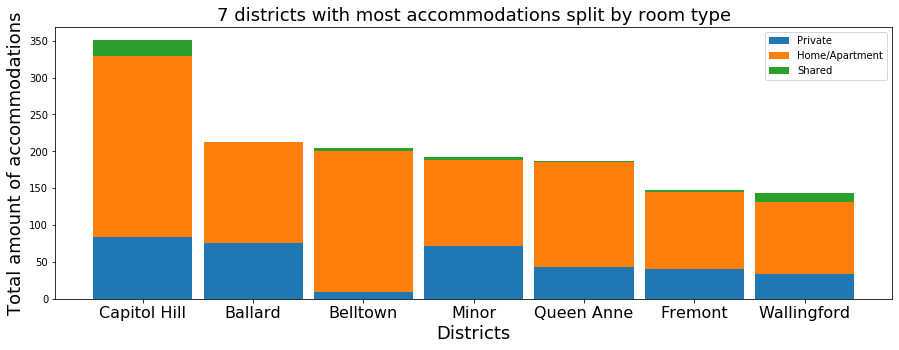
\includegraphics[width=3.5in]{photo/4_most_acc_split_by_roomtype.png}\\
  \caption{ten districts with most accommodations split by room type}\label{districts_room_types}
  \end{center}
\end{figure}
\subsubsection{Reviews}
%
In order to have an insight whether the reviews are written by satisfied or rather unsatisfied visitors, we computed a bar chart which shows the rating-number of reviews ratio. (Figure \ref{score_reviews_ratio})
%
%Figure
\begin{figure}
  \begin{center}
  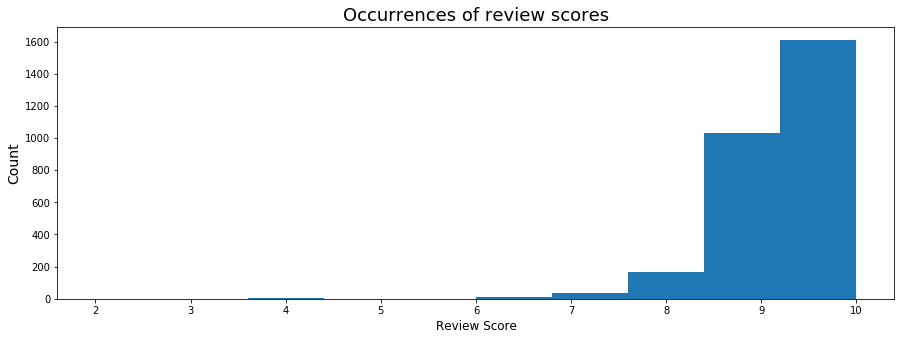
\includegraphics[width=3.5in]{photo/2_1_occurences_of_review_scores.png}\\
  \caption{Score and number of reviews ratio}\label{score_reviews_ratio}
  \end{center}
\end{figure}
%

Besides, it shows that most of the reviews give the highest value possible (10) and there are hardly no reviews that give a rating value lower than 8. So, in our further analysis we assume that the reviews are written in a rather positive tone and we need to keep in mind that the reviews have been written by overall satisfied tourists.
=======
Besides, it shows that most of the reviews give the highest value possible (10) and there are hardly no reviews that give a rating value lower than 8. \\
First we had the idea of creating a new feature called \textit{Sentiment} for each review. It should be calculated with a Sentiment Analysis and label each review with a score. By reading related work to the Seattle-Dataset, we noticed that another group already research this idea. They used the Microsoft Azure Sentiment Analysis API to label each review with a score between 0 to 100. Unfortunately they gained the information in the Data section that this feature has no revelant effect on the prediction for the price \cite{RN1}, because as shown in figure \ref{score_reviews_ratio}, there is no Gaussian-Distribution or any other useful distribution for the reviews. \\

So, in our further analysis we assume that the reviews are written in a rather positive tone and we need to keep in mind that the reviews have been written by overall satisfied tourists.
>>>>>>> 3dcb1543e0f90a38b0ebc0696dfa9a29e17291fb
In order to make sure that there is no correlation between the number of reviews and the review score of apartments in a certain neighborhood, we generated a figure which shows that relationship (Figure \ref{compare_the_neighbourhoods}).
%
%Figure
\begin{figure}
  \begin{center}
  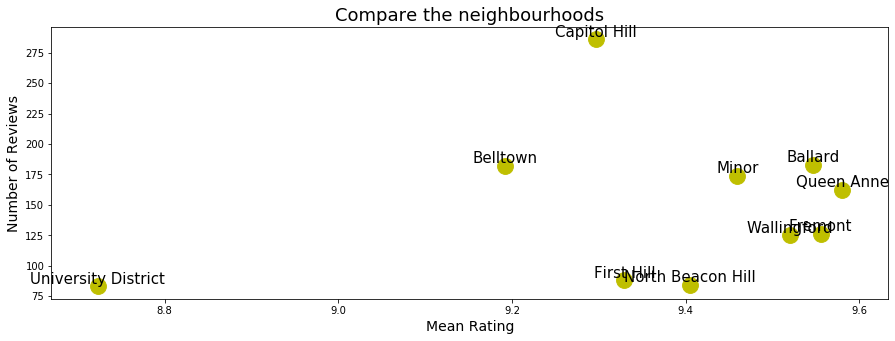
\includegraphics[width=3.5in]{photo/2_2_compare_the_neighbourhoods.png}\\
  \caption{Mean rating and number of reviews ratio (per neighborhood)}\label{compare_the_neighbourhoods}
  \end{center}
\end{figure}
%
In this figure it becomes visible that neighborhoods, whose apartments in total got 50 to 100 reviews score a mean rating of about 9.2 to 9.7. Approximately the same mean rating is also achieved by district where the apartments are rated 125 to 300 times. There is only one outlier (‘University District’), which scored al pretty low mean rating value compared to all other districts. As this is the only outlier, we will neglect this in our following assumptions.
To sum up, we can conclude that both figures (\ref{score_reviews_ratio_neighborhood} and \ref{score_reviews_ratio}) show that the mean rating for every district is relatively high and a high value is not dependent on the number of reviews for a certain district.
\subsubsection{Calendar}
This part of the data shows, when certain apartments are available and when they are rented out. Within our analysis we assume, that an apartment, which is listed as ‘not available’ in the ‘calender.csv’ is occupied by a visitor. If it is ‘available’ we assume that the owners would have liked to rent the apartment out but there has not been any visitor renting it. In figure \ref{occupied_ratio_appartments} the ratio of occupied and available apartments in 2016 is presented.
%
%Figure
\begin{figure}
  \begin{center}
  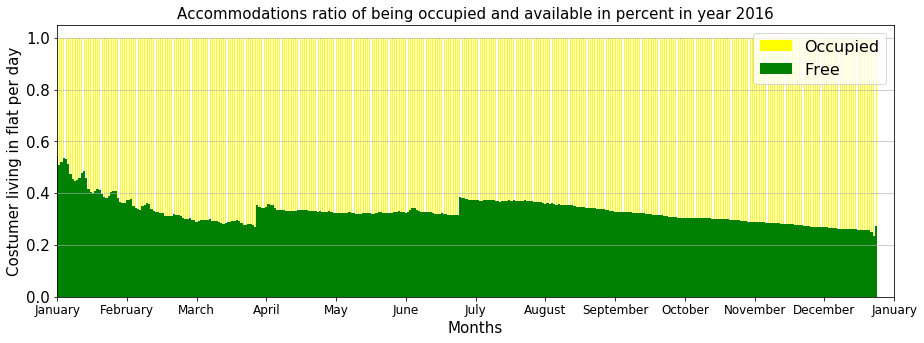
\includegraphics[width=3.5in]{photo/11_acc_ratio_occupied.png}\\
  \caption{occupied ratio of appartments}\label{occupied_ratio_appartments}
  \end{center}
\end{figure}
%
While in January only half of the apartments have been occupied, the number of rented apartments raised until April when a sudden drop in rented apartments appeared. The same procedure repeats in July. After that second drop the number of occupied accommodations raises again. Nevertheless, it has to be mentioned that the percentage of free apartments never exceeds 40\% after February anymore but also never drops below 20\%. At this point the question, whether there is a correlation between the degree of booking and a ‘perfect’ description exists and therefore the percentage of free apartments can be decreased by mentioning the right aspects in the description. 

\section{Models}

As the team of this paper \cite{RN1} mentioned in their average listing price per neighbourhood, they figured out that the neighbourhood has a huge impace on the price prediction. The main focus of our project was not the price prediction, but we tried to reach similar results. Our best mean absolute error is the linear regression with 43.89\$ \ref{linear_regression}. The neural network scores best for their prediction with a score of 35–32\$ \cite{RN1}. \\
We didn't have the capacity to transform the categorical neighbourhood feature into a numerical one and try-out multiple neural networks. \\
Our deviation of 10\$ from their best result can be explained by that.

\subsection{Natural Language Processing}
NLP stands for natural language processing. We can use this technique to process and analyze natural language data from the reviews of our dataset. NLP breaks down language into tinier, elemental pieces, trying to understand the relationships between the pieces and explore how the pieces are related together to generate meanings and conclusions out of it. To perform analysis, we encounter plenty of steps called the preprocessing. Most of this steps can be solved with multiple python packages. We decided to use the NLTK package, because it provides an easy to use dashboard and contains all of the required preprocessing methods.
The preprocessing steps for transforming the reviews into Wordclouds are below with exactly this sequence of steps:
\begin{itemize}
 \item Regular Expression Tokenizer
 \item Stopwords for English + two additional Words “Seattle” and “Neighbourhood”
 \item Lowercase
 \item WordNetLemmatizer
\end{itemize}

\subsubsection{Regular Expression Tokenizer}
This  tokenizer uses a regular expression term with the intention of cleaning the text completely from any punctuation marks and unnecessary spaces.  The expression r'\textbackslash +' does exactly this, because it avoids every character which is not alphanumeric (A-Z, numbers) and underscore (\_) or an asterisk (*). Everything else will get omitted by the regular expression. The Tokenizer itself detects the ASCII character for the space and splits in this way the words from each other to store it in an array.

\subsubsection{Stop Words}
A Text normally contains stop words like ‘the’, ‘is’, ‘are’. Stop words should be filtered from the text to be processed in the best way. There is not an universal list of stop words in NLP research, however the nltk module contains a list of stop words.

\subsubsection{Lowercase}
This is just the built-in pyton method .lower() which can be used to turn strings into lowercase.

\subsubsection{WordNetLemmatizer}
Lemmatization is the process of turning the words into their base form. There is a second almost similar approach called stemming. 
The difference between stemming and lemmatization is, lemmatization looks at the context oft he word and transforms it to its base form, whereas stemming just removes the last few characters. Unfortunately this often leads to incorrect spelling and meaning errors. For example, lemmatization would properly identify the base form of ‘caring‘ to ‘care’, whereas, stemming would cutoff the ‘ing’ part and convert it to car.
\begin{itemize}
\item Caring with \textit{Lemmatization} into Care
\item Caring with \textit{Stemming} into Car
\end{itemize}
\subsection{Linear Regression}
Dr Liu described the Linear Regression as one of the most widely used techniuqes for advanced predictions. It is fundamental to more complex models, easy to interpret and easy to solve. \cite{RN7}
Linear regression attempts to model the relationship between two variables by fitting a linear equation to observed data.
The fitted line can mathematically described as:
\begin{equation}
Y_i = \beta_0 + \beta_1 X_i + \epsilon_i
\end{equation}

\begin{figure}
  \begin{center}
  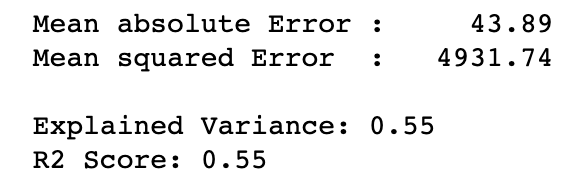
\includegraphics[width=3.5in]{photo/linear_regression.png}\\
  \caption{Errors of the Linear Regression}\label{linear_regression}
  \end{center}
\end{figure}

\subsection{Extra Tree Classifier }
The Extra Tree Classifier is a model derived from the random forest model. Decision Trees are the fundamental components of Random Forests.  Aurélien Géron says that Random Forests are among the most powerful Machine Learning algorithms available \cite{ho} . We are using it to classify the feature importance. Based on Entropy and the Information Gain, we get the essential feature\cite{BernardChiu} \cite{decisionforests}. Entropy and Information are defined by: 
\begin{equation}
Entropy: H(X) = -\sum p(X)\log p(X) 
\end{equation}
\begin{equation}
Information Gain: I(X,Y)= H(X)-H(X|Y)
\end{equation}
In other words, we get the feature which organises the data the most. 

The features with the according entropy are shown in figure \ref{feature_importance}

\begin{figure}
  \begin{center}
  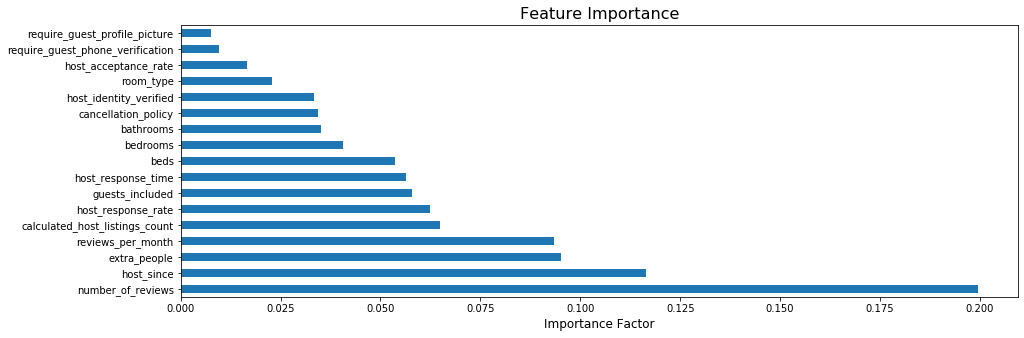
\includegraphics[width=3.5in]{photo/7_feature_importance.png}\\
  \caption{Feature Importance}\label{feature_importance}
  \end{center}
\end{figure}

This leads to the conclusion, that first leafs for predicting the price with a Tree-Classifier should be the amount of reviews. 

\begin{figure}
  \begin{center}
  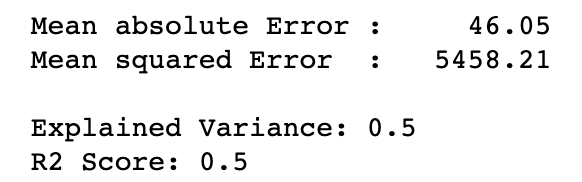
\includegraphics[width=3.5in]{photo/elastic_net.png}\\
  \caption{Errors of the Elastic Net}\label{elastic_net}
  \end{center}
\end{figure}

\subsection{Elastic Net CV}
\subsection{Multinomial Naive Bayes}
\subsection{LSTM Neuronal Network}



\section{Analysis}
\subsection{Which facts lessors need to address in their description to raise the interest of potential customer, who ‘fit’ the vibe of the neighborhood and set their focus on the same aspects as former customers of these apartments?}
In order to know what words the lessors are supposed to use in the description, we take a look at the reviews with a wordcloud. The bigger the words in the wordcloud, the more often the word was used. For example, if the customers often write the word walk in the reviews due to informing what was in walking distance of the Airbnb, the work walk will be big in the wordcloud. 
To answer this question the six most reviewed cities Capitol Hill, Ballard, Queen Anne, Belltown, Minor, Wallingford were analyzed. First, you can see that all cities have the words walk, park and restaurant written in big. The word “downtown” is also used often. For minor, the word “lake” is very important. The rest of the words indicate that words like minute, shop, market are used often by customers. Interestingly, the word “Washington” is important for the cities Minor and Capitol Hill.


\subsection{Which factors did influence the degree of booking of former rented apartments? }
In order to answer this question, the Extra Tree Classifier was used. With the help of the Extra Tree Classifier one can see the feature importance. According to the feature importance the number of reviews influences the degree of booking of former rented apartments the most. Customers also care about how long the host has been on the platform and extra people. Almost equally as important are the number of reviews per month. This underlines how important the reviews are. The amount of host listings, the response rate and what is included for the guests influences the results of ones booking almost on the same level. The host should also care about the response rate and the number of beds as the next important thing on the list. Less important are the cancellation policy, bedrooms, bathrooms and if the host is verified on Airbnb. The Room type, host acceptance rate, phone verification and if the host has a profile picture are the least important factors influencing the degree of booking the apartments.
\subsection{Which price can be charged for an apartment with certain characteristics?}
First of all, we created a Linear Regression model in order to predict the price influenced by all other attributes. For this prediction we achieved a Mean Absolute Error of 44.28, which is, taking into account that the minimum rent is 10 dollar and maximum rent per night 1,650\$, very low. Therefore, we can assume that the listed attributes have a significant impact on the price of an accommodation and it is possible to estimate the rental price by these attributes and therefore it makes sense to use a classification tree, which takes these attributes into account.
Figure Linear regression
In the following, we use the Extra Tree Classifier in order to find out, which attributes have a strong correlation with the price and therefore influence the price of an apartment the most. A classification tree uses the values of attributes to create groups, in which all the apartments have the same (or at least similar) values for the attributes. According to our analysis, the attributes with the highest influence on the price have a correlation coefficient in a range of 0.01 and 0.2. The highest influence on the price is the number of reviews an apartment has. This attribute has a correlation of approximately 20\%, which is almost twice as much as the second important attribute has by showing 0.112 as correlation coefficient. This attribute indicates how long the lessor is already registered as host on Airbnb. As third important factor, with a correlation coefficient of a little bit less than 0.1 the number of extra people influences the price. Other attributes which influence the price are for example the number of listings a host has/ had, number of beds, number of bath- and bedrooms. The least significant attribute in our visualization is, whether the guest needs a profile picture (with a coefficient of about 0.01). (Figure \ref{correlation-attribute-price})
\begin{figure}
  \begin{center}
  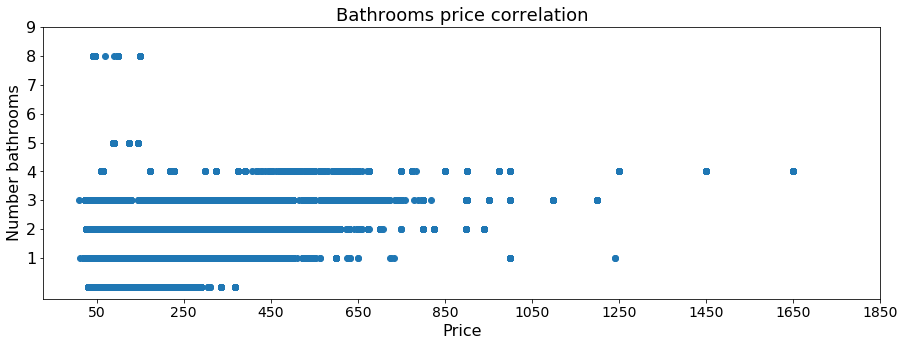
\includegraphics[width=3.5in]{photo/9_bathroom_price_correlation.png}\\
  \caption{Correlation attribute-price}\label{correlation-attribute-price}
  \end{center}
\end{figure}
In order to check that all the attributes only determine the price and do not have an influence on the price via another attribute, we also compute a heatmap to see the correlation of attributes among each other. This visualizes that host-response-time, host-response-rate and host-acceptance-rate correlate with each other and also the number of bedrooms, bathrooms and beds. So, these attributes groups influence each other and their impact on the price should be considered in a group. Furthermore, we can mention that the number of bathrooms, bedrooms and beds influence each other. So, a lessor should also take into account that if an apartment has for example a high number of bedrooms then also the number of bathrooms is high. According to this a lessor can also get some indication for the price he can charge. If his apartment has many bedrooms but only one bathroom, he can assume that other accommodations with the same number of bedrooms has more bathroom and therefore can also charge a higher price. So, this correlation is interesting for the lessors to get some price indication. (Figure \ref{heatmap })
\begin{figure}
  \begin{center}
  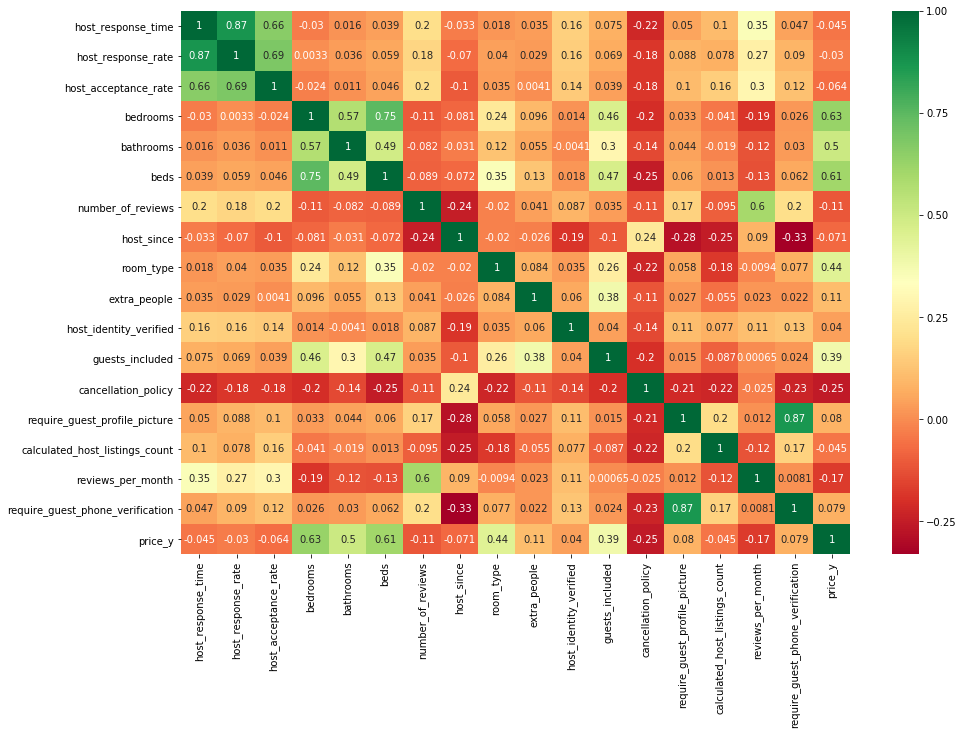
\includegraphics[width=3.5in]{photo/8_heatmap.png}\\
  \caption{Correlation attribute-price}\label{heatmap }
  \end{center}
\end{figure}
So, if a lessor wants to (re)determine the price for his accommodation, he first of all needs to consider how many reviews he got so far for the apartment. (Note: As we noted before, the reviews all give a high rating, so they are all positive. Taking this into account, it is very likely that the lessor needs to check the number of positive reviews for determining the price.) Furthermore, the lessor needs to consider how long he is already registered as host and how many people can stay in the apartment. If he considers the impact of the number of bedrooms, bathrooms and beds, he should also take into account, the correlation of the three attributes among each other.
As we already saw in figure \ref{correlation-attribute-price}, the number of beds, bedrooms and bathrooms do not have the highest impact on the price although somebody might expect, that the price is strongly influenced by these factors. \\
The same result was already shown by another paper, which further proofs those relevant features \cite{RN1}. 

By having a closer look on the correlation between the number of bathrooms and the price as well as the number of bathroom and price, it can be recognized that an increasing number of bed- and bathrooms does not increase the entry level price within this group but only the maximal price increases. So, it is possible to find an accommodation with a different amount of bath-/ bedroom for a price of 50 dollar per night. This changes if the number of bedrooms exceeds 5. Then there is also an increase of the entry level price visible. We can conclude that the price of an apartment is probably more influenced by the fact whether it has less or more than 5 bedrooms or not. (Figure \ref{bedroom-price-correlation})
\begin{figure}
  \begin{center}
  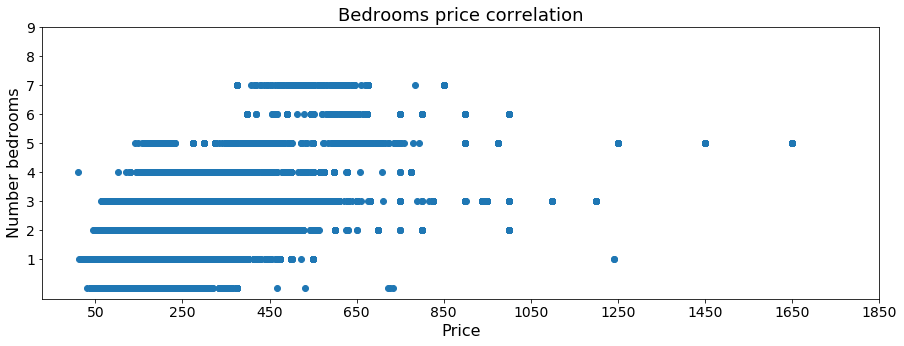
\includegraphics[width=3.5in]{photo/10_bedrooms_price_correlation.png}\\
  \caption{number-of-bedroom-price-correlation}\label{bedroom-price-correlation}
  \end{center}
\end{figure}
The same change can also be seen for the correlation of bathrooms and price but the change of the entry level is not that big. Therefore, the ‘strong’ change in the entry level price becomes already visible for 4 bathrooms. (Figure \ref{bathrooms-price-correlation})
\begin{figure}
  \begin{center}
  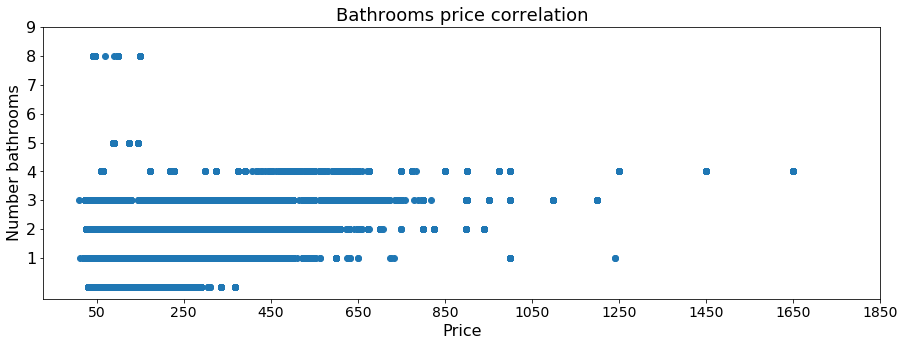
\includegraphics[width=3.5in]{photo/9_bathroom_price_correlation.png}\\
  \caption{number of bathrooms price correlation}\label{bathrooms-price-correlation}
  \end{center}
\end{figure}

\subsection{When can lessors increase the price per night for their apartment and when should they lower it?}
To answer this question, we want to predict the price changes for 2017. First of all, we started by checking out the change of mean flat prices in 2016 (Figure \ref{correlation-attribute-price}). 
Prices increase from January to July form about 120 to 150 dollar and decrease until November to 135 dollar. During the last month prices slightly start to increase again. It can be seen that the correlation between charged prices and the occupation ratio is rather low, as the first drop of the occupation ratio in April does not reflect in a price drop. Nevertheless, the second decrease in the number of rented apartments does reflect in the charged prices as also the price curve decreases after July. But during the month of December, prices increase as well as the number of free apartments decrease. This irregularity might be due to the fact that many people travel during Christmas time and therefore their willingness to pay is slightly increased. 

\subsection{What is a good point in time to start a marketing campaign?}
In order to find the right point in time to start a marketing campaign, we need to know, during which periods the number of visitors decreases. To get some good results, we plotted a graph showing the number of visitors according to the time.
In Figure 5.2 it can be seen that the number of visitors fluctuates very strong also within a month. This might be caused by changes within a week, as usually on weekends more people consider to travel and therefore more apartments are rented as well as public holidays influence the number of tourists. As exactly reflecting this fluctuation in a model would lead to a very complex model, which is expensive to create and the risk of a model overfit becomes very high, we use Linear Regression to reflect the trend of 2016 and in a second step predict the numbers of visitors for 2017. We can see that the number of visitors decreases between January and March and increases between March and July. After that there is a decrease until December. Nevertheless, the fluctuation is about 200 visitors. Compared to a total number of over 2400 visitors this change is quite small.
The predicted number of visitors can be seen in Figure 5.3.

For 2017 it is predicted that the number of visitors raises from January to March and decreases until July. For the rest of the Year the number of visitors will raise again. So, the best point in time to start a marketing campaign would be during February till March. As the number of visitors will fall from March to July, the marketing campaign should prevent this. A campaign usually needs some time until its effectiveness can be seen so it should be started earlier than the actual decrease takes place and when the predicted decrease should take place, the effect of the campaign should keep the number of visitors on the level of March or even increase it. The campaign could be stopped in August, as its effect will last a little bit longer and between September and October the number of visitors will be on the level of March again without any campaign.


%
\section{Your findings and impacts}
We want to improve the effectiveness of marketing for Airbnb Seattle based on our findings. This can be beneficial for the lessors and Airbnb itself as Airbnb makes money off of the lessors. That means, Airbnb is only profitable if the lessors are able to rent out their listings. As a consequence, Airbnb should help the lessors to attract more visitors. 
\\
Referring to the previous analysis one can see that the reviews are the most important factor of the consumers decision. That means the more reviews the lessors have the higher the chance their listings gets rented. This is why the lessors and Airbnb should ask their renters to write a review after they leave in order to attract more people. One should keep in mind that this report is only considering positive reviews. \\
Another suggestion for the lessors is to update their description with places that are in walking distance. Places that the renters want to visit might be shops, the metro, parks, downtown, etc. One can also mention where the renters can get food with mentioning where the nearest restaurants or cafes are. The bottom line is, the lessors should put every place into the description that is in walking distance. \\
As mentioned before, the number of reviews plays a huge part in whether a listing gets booked or not and how much can be charged. Another big factor is how long the host has been active and how many listings the host has. As those are qualities that can only be build over time, older hosts get rewarded and can charge more per listing. Consequently, lessors need to be patient in order to show that they are reliable and grow their credibility. This way their listings will get booked more often and they can charge a higher price. \\
Newer hosts can try to focus on their host\_response\_time, host\_response\_rate and host\_acceptance\_rate. As qualities like number of reviews, number of listings and how long the host has been active needs time, these are factors lessors can work on immediately in order to rent out their listing for a higher price. \\
If the host has the chance, then it is worth considering that higher number of bedrooms, bathrooms and beds can lead to people willing to pay more for the listing. That can be due to people renting the place to explore the city or work most of the time and only wanting a place to stay and shower at. This gives a reason to suspect that renters will not spend a lot of time in the Airbnb. 
We already know that the number of visitors fluctuates a lot within a month. This can be due to people visiting new places over the weekend. Consequently, it would be profitable to increase the prices from Friday to Sunday and lower them from Monday to Thursday. Moreover, it makes sense to keep the prices low from January to March before slowly increasing them from March to September. July should be the most expensive month. In December the prices can be increased again. That can be a result of holidays. Because many people decide to visit their families or go on vacation during their holidays, the demand for places to stay increases during that time period. \\
As Airbnb itself profits form their lessors renting out their places, it would be interesting to know how they can help their lessors. One way is to start campaigning at the right moment. According to the analysis, in the year 2017 the number of visitors will decrease from March to July. Meaning the marketing campaign should start in February and end in August. As Airbnb is an online platform the advertisements should be online as well. This way, possible visitors can be reached who already are comfortable using the internet. 

%
\section{Conclusion}
ToDo



\section*{Acknowledgment}
The authors would like to thank Dr. Liu for really good supervising of our group. Dr. Liu helped us so much and we wouldn't have reached this result without him. 



% if have a single appendix:
%\appendix[Proof of the Zonklar Equations]
% or
%\appendix  % for no appendix heading
% do not use \section anymore after \appendix, only \section*
% is possibly needed

% use appendices with more than one appendix
% then use \section to start each appendix
% you must declare a \section before using any
% \subsection or using \label (\appendices by itself
% starts a section numbered zero.)
%

% ============================================
%\appendices
%\section{Proof of the First Zonklar Equation}
%Appendix one text goes here %\cite{Roberg2010}.

% you can choose not to have a title for an appendix
% if you want by leaving the argument blank
%\section{}
%Appendix two text goes here.


% use section* for acknowledgement
%\section*{Acknowledgment}


%The authors would like to thank D. Root for the loan of the SWAP. The SWAP that can ONLY be usefull in Boulder...


% Can use something like this to put references on a page
% by themselves when using endfloat and the captionsoff option.
\ifCLASSOPTIONcaptionsoff
  \newpage
\fi



% trigger a \newpage just before the given reference
% number - used to balance the columns on the last page
% adjust value as needed - may need to be readjusted if
% the document is modified later
%\IEEEtriggeratref{8}
% The "triggered" command can be changed if desired:
%\IEEEtriggercmd{\enlargethispage{-5in}}

% ====== REFERENCE SECTION

%\begin{thebibliography}{1}

% IEEEabrv,

\bibliographystyle{IEEEtran}
\bibliography{IEEEabrv,Bibliography}
%\end{thebibliography}
% biography section
% 
% If you have an EPS/PDF photo (graphicx package needed) extra braces are
% needed around the contents of the optional argument to biography to prevent
% the LaTeX parser from getting confused when it sees the complicated
% \includegraphics command within an optional argument. (You could create
% your own custom macro containing the \includegraphics command to make things
% simpler here.)
%\begin{biography}[{\includegraphics[width=1in,height=1.25in,clip,keepaspectratio]{mshell}}]{Michael Shell}
% or if you just want to reserve a space for a photo:

% ==== SWITCH OFF the BIO for submission
% ==== SWITCH OFF the BIO for submission


%% if you will not have a photo at all:
%\begin{IEEEbiographynophoto}{Ignacio Ramos}
%(S'12) received the B.S. degree in electrical engineering from the University of Illinois at Chicago in 2009, and is currently working toward the Ph.D. degree at the University of Colorado at Boulder. From 2009 to 2011, he was with the Power and Electronic Systems Department at Raytheon IDS, Sudbury, MA. His research interests include high-efficiency microwave power amplifiers, microwave DC/DC converters, radar systems, and wireless power transmission.
%\end{IEEEbiographynophoto}

%% insert where needed to balance the two columns on the last page with
%% biographies
%%\newpage

%\begin{IEEEbiographynophoto}{Jane Doe}
%Biography text here.
%\end{IEEEbiographynophoto}
% ==== SWITCH OFF the BIO for submission
% ==== SWITCH OFF the BIO for submission



% You can push biographies down or up by placing
% a \vfill before or after them. The appropriate
% use of \vfill depends on what kind of text is
% on the last page and whether or not the columns
% are being equalized.

\vfill

% Can be used to pull up biographies so that the bottom of the last one
% is flush with the other column.
%\enlargethispage{-5in}



% that's all folks
\end{document}
